\section{Results}

The results from our simulation study are shown in figure \ref{fig:simulation-results}. The precision of the estimate of effect of concomitant drug use increases as the number of repeatedly sampled (and sparsely sampled) patients increases.  Shown in red are the sample means of the 10 runs (black dots).  On average we see a small amount of bias in the estimates.  This is expected since the sparsity inducing priors have the majority of their density in a small neighbourhood of 0, regularizing effects towards 0.  For purposes of discovery, these biases may be acceptable if the result is a decrease in model variability.



\begin{table}
	
	\caption{\label{tab:table-1}Descriptive statistics for repeatedly sampled and sparsely sampled data.  Note, amiodarone is a CYP3A4 inhibitor.  The study which generated repeatedly sampled data excluded any patients whom were taking CYP3A4 inhibitors, so all patients in the repeatedly sampled data are assigned a value of 0 for concomitant amiodarone.}
	\centering
	\begin{tabular}[t]{llll}
		\toprule
		& Repeatedly Sampled Data & Sparsely Sampled Data & Overall\\
		\midrule
		& (N=36) & (N=401) & (N=437)\\
		\addlinespace[0.3em]
		\multicolumn{4}{l}{\textbf{Age}}\\
		\hspace{1em}Mean (SD) & 49.8 (11.5) & 78.8 (9.43) & 76.4 (12.5)\\
		\hspace{1em}Median [Min, Max] & 50.0 [26.0, 70.0] & 79.0 [47.0, 98.0] & 79.0 [26.0, 98.0]\\
		\addlinespace[0.3em]
		\multicolumn{4}{l}{\textbf{Weight (kg)}}\\
		\hspace{1em}Mean (SD) & 88.0 (24.4) & 85.6 (23.8) & 85.8 (23.8)\\
		\hspace{1em}Median [Min, Max] & 83.5 [54.7, 137] & 81.6 [40.0, 221] & 81.8 [40.0, 221]\\
		\addlinespace[0.3em]
		\multicolumn{4}{l}{\textbf{Creatinine (micromol/L)}}\\
		\hspace{1em}Mean (SD) & 68.0 (12.5) & 105 (44.5) & 102 (43.9)\\
		\hspace{1em}Median [Min, Max] & 65.0 [50.0, 95.0] & 92.0 [42.0, 316] & 89.0 [42.0, 316]\\
		\addlinespace[0.3em]
		\multicolumn{4}{l}{\textbf{Sex}}\\
		\hspace{1em}female & 23 (63.9\%) & 178 (44.4\%) & 201 (46.0\%)\\
		\hspace{1em}male & 13 (36.1\%) & 223 (55.6\%) & 236 (54.0\%)\\
		\addlinespace[0.3em]
		\multicolumn{4}{l}{\textbf{Concomitant Amiodrone (mg/day)}}\\
		\hspace{1em}Mean (SD) & 0 (0) & 16.2 (60.1) & 14.9 (57.7)\\
		\hspace{1em}Median [Min, Max] & 0 [0, 0] & 0 [0, 400] & 0 [0, 400]\\
		\bottomrule
	\end{tabular}
\end{table}


\begin{figure}
	
	{\centering 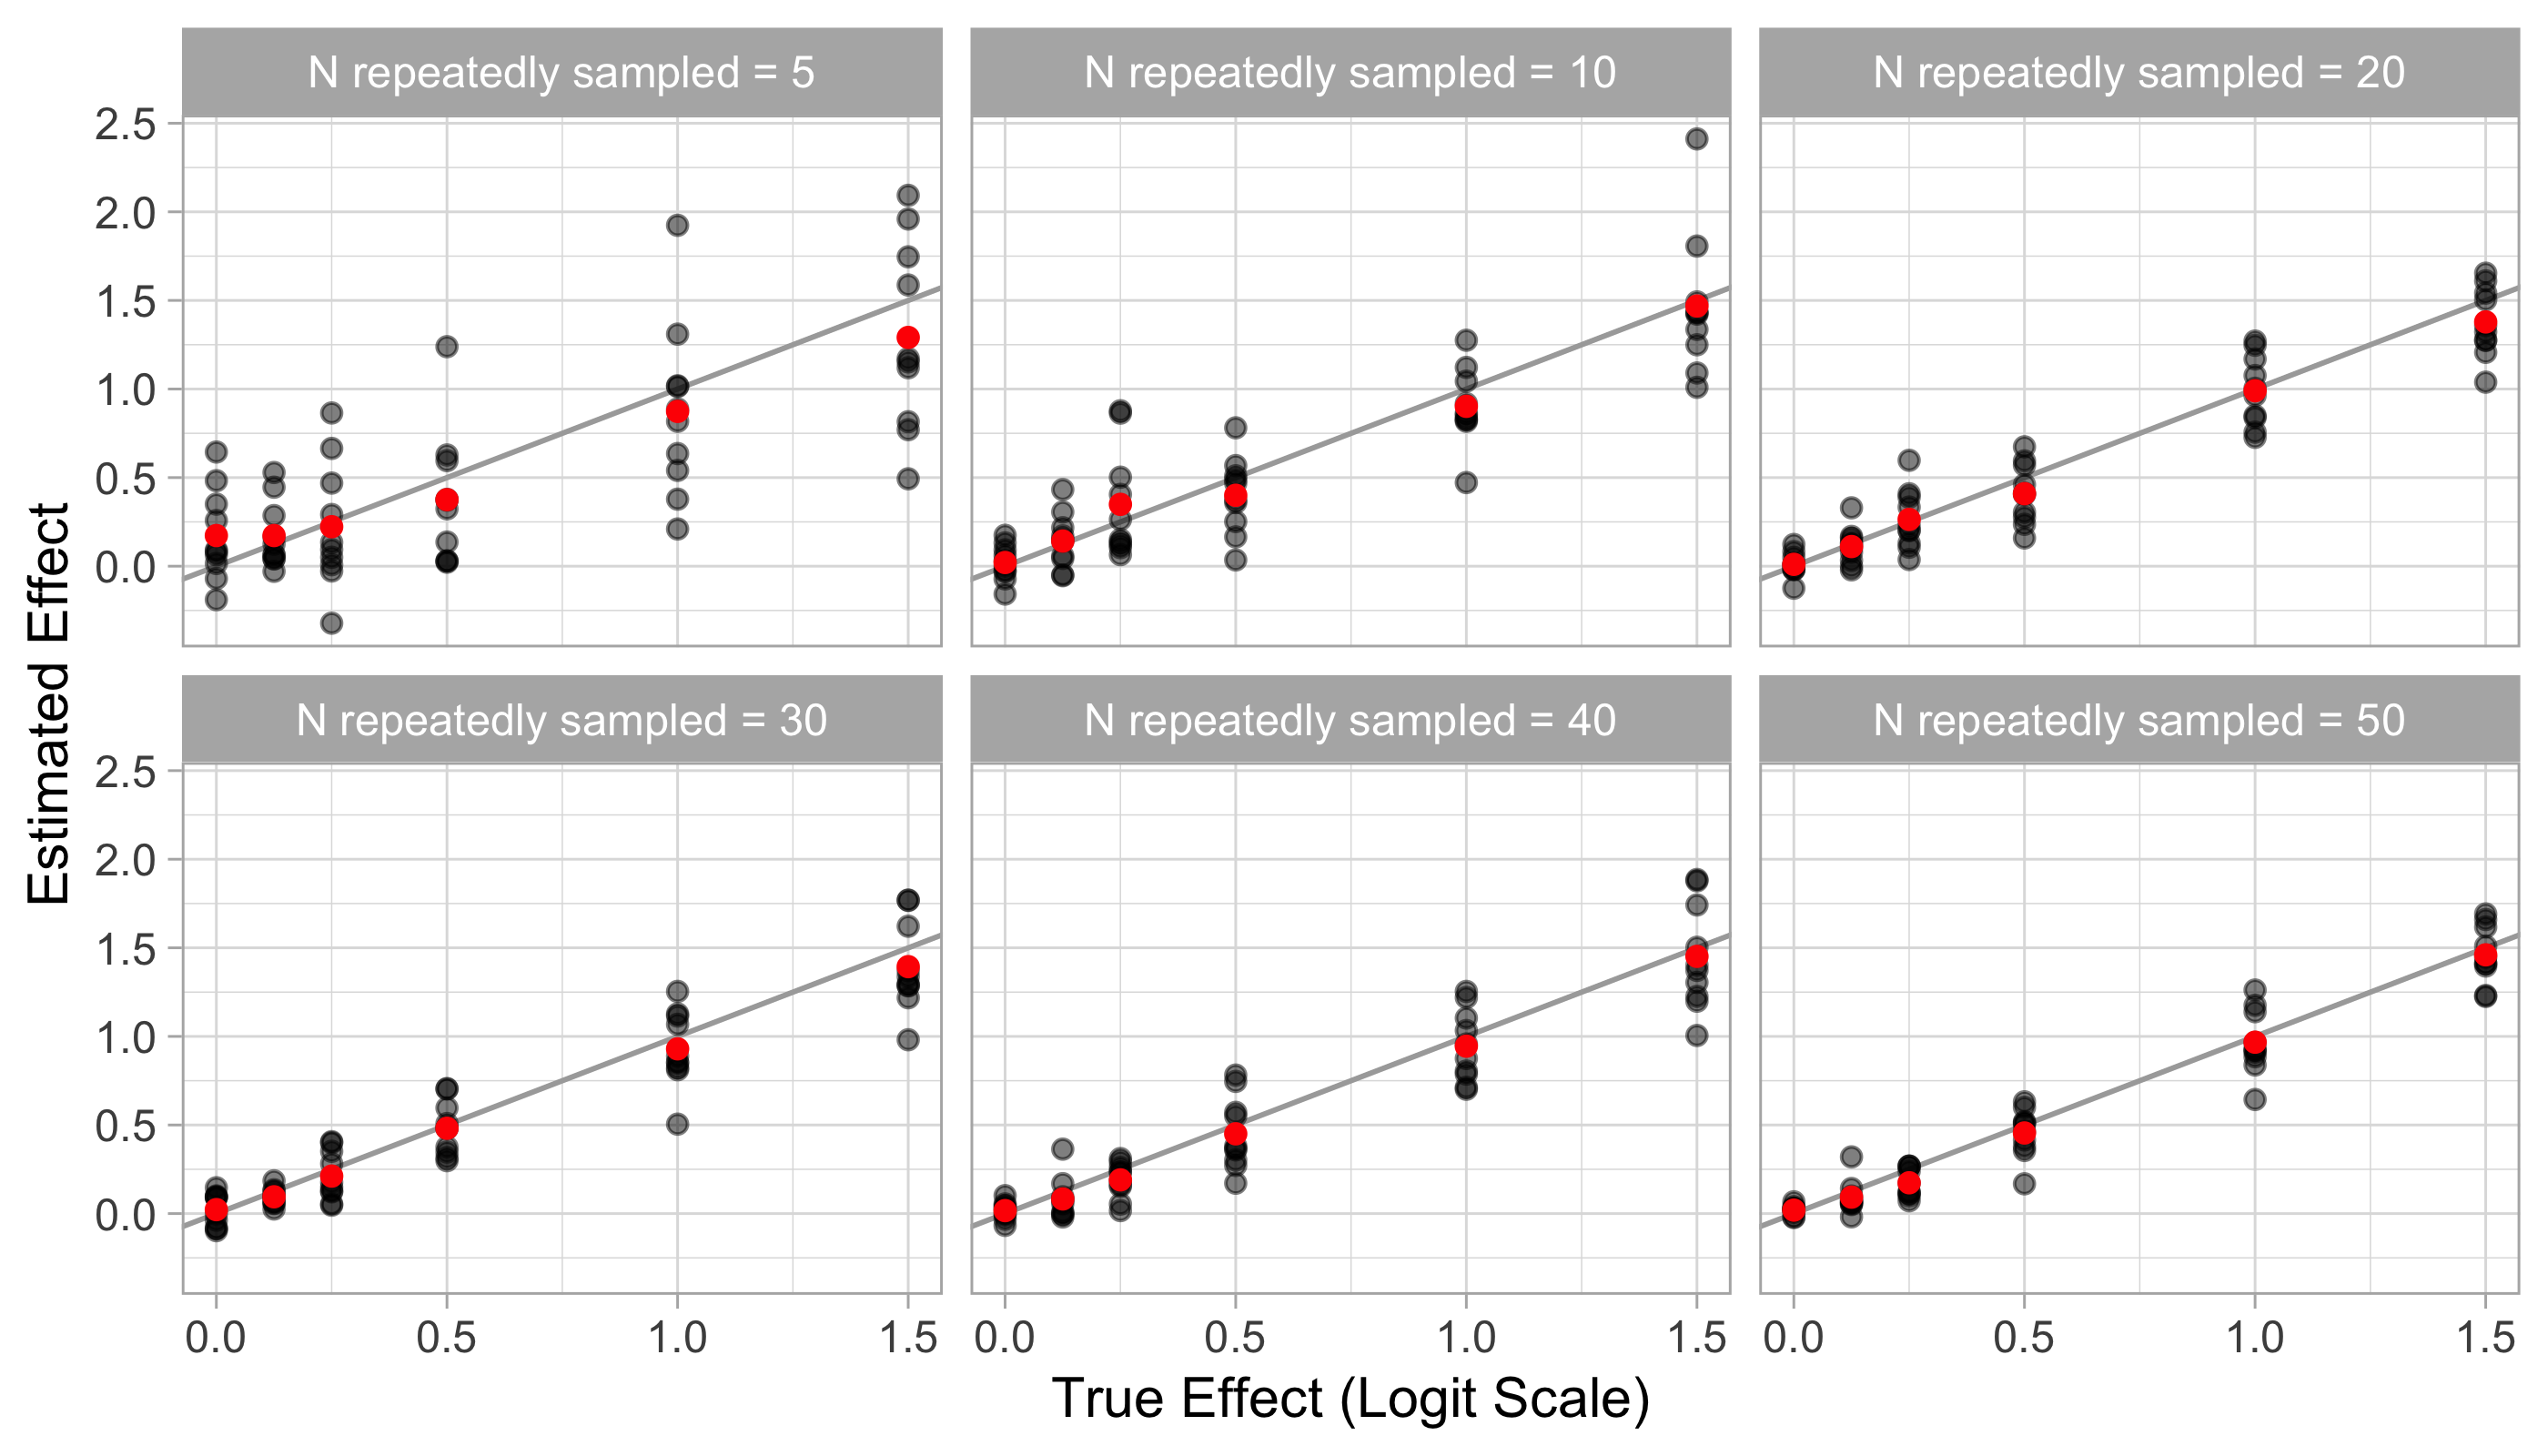
\includegraphics[width=\linewidth]{figures/simulation-results-1} 
		
	}
	
	\caption{Results from our simulation study.  Black dots represent the estimated effect of a novel predictor.  Red dots indicate the average estimate across the 10 repetitions. Data are faceted by the number of repeatedly sampled patients.  Smaller datasets show more bias towards the null.  This bias attenuates as sample size increases.}\label{fig:simulation-results}
\end{figure}


When using real data, our model can accurately predict both repeatedly
sampled and sparsely sampled data. Shown in figure
\ref{fig:plot-model-predictions} is a log-log plot of predicted and
actual concentrations for both datasets. The model makes more accurate
predictions for repeatedly sampled patients (because it is able to
estimate the random effect in each pharmacokinetic parameter). The
apparent increase in prediction error for the sparsely sampled can be
explained by the absence of random effects for each patient. The within
and between patient variation manifests as measurement error solely,
thus leading to lower predictive ability.

With a model for the pharmacokinetics of apixaban in hand, estimates of
salient pharmacokinetic phenomena can be easily obtained. In figure
\ref{fig:max-concentration}, we use our model to estimate the max
concentration for the reference patient under different doses of
amiodarone. Through our model, we estimate concomitant amiodarone
increases bioavailability, which in turn increases max concentration.
Shown in black is the expected max concentration conditioned on
concomitant amiodarone dose, as well as 95\% equal tailed posterior
credible intervals.

Additionally, we contrast the pooled model's estimates of covariate
effects with estimates from model's fit to either the sparse or
repeatedly sampled data. Marginal posterior densities for the effects of
covariates on the pharmacokientic parameters are shown in figure
\ref{fig:effect-estimates}. In most cases, the effects seem to have
higher precision due to the increase in sample size, and generally there
is no large disagreement in either sign or magnitude of effect
estimates.



\begin{figure}
	
	{\centering 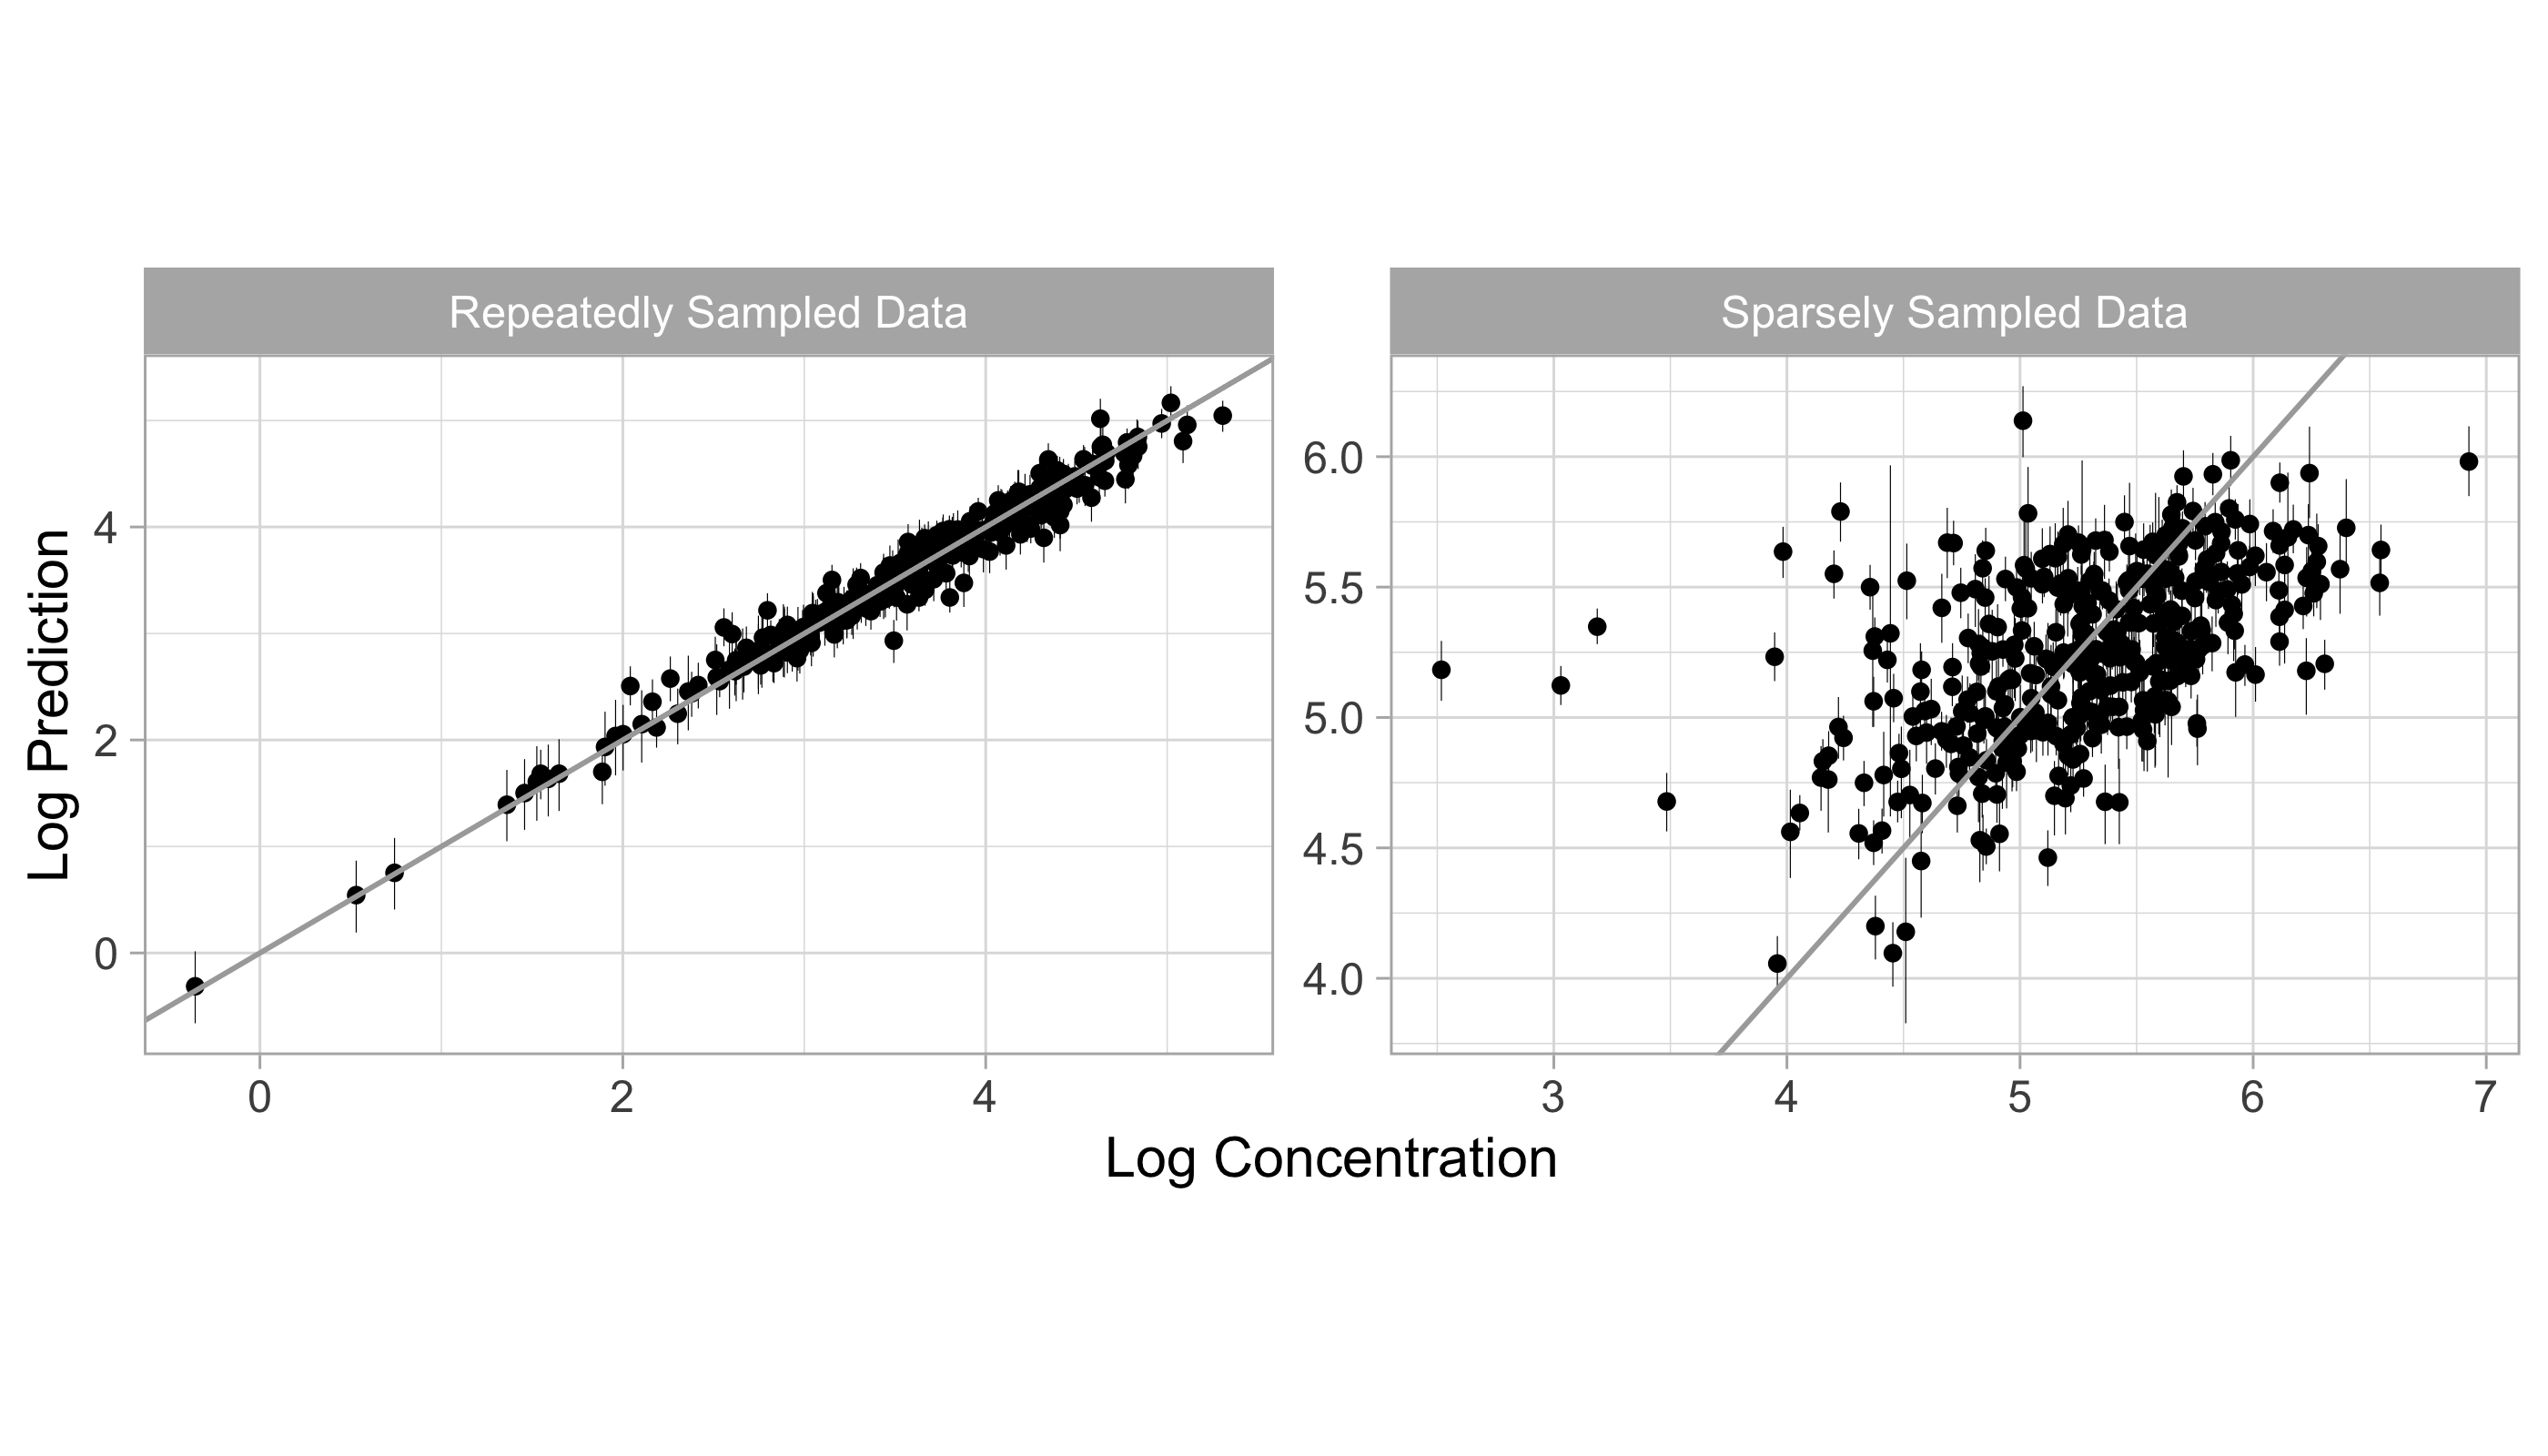
\includegraphics[width=\linewidth]{figures/plot-model-predictions-1} 
		
	}
	
	\caption{Predicted vs observed concentrations for both datasets on the log scale. Note each plot has a separate scale. Sparsely sampled data can not be predicted as accurately as the repeatedly sampled data, due in part to the inability to estimate patient random effects in pharmacokinetic parameters.  This additional variance left unexplained manifests as measurement error.}\label{fig:plot-model-predictions}
\end{figure}

\begin{figure}
	
	{\centering 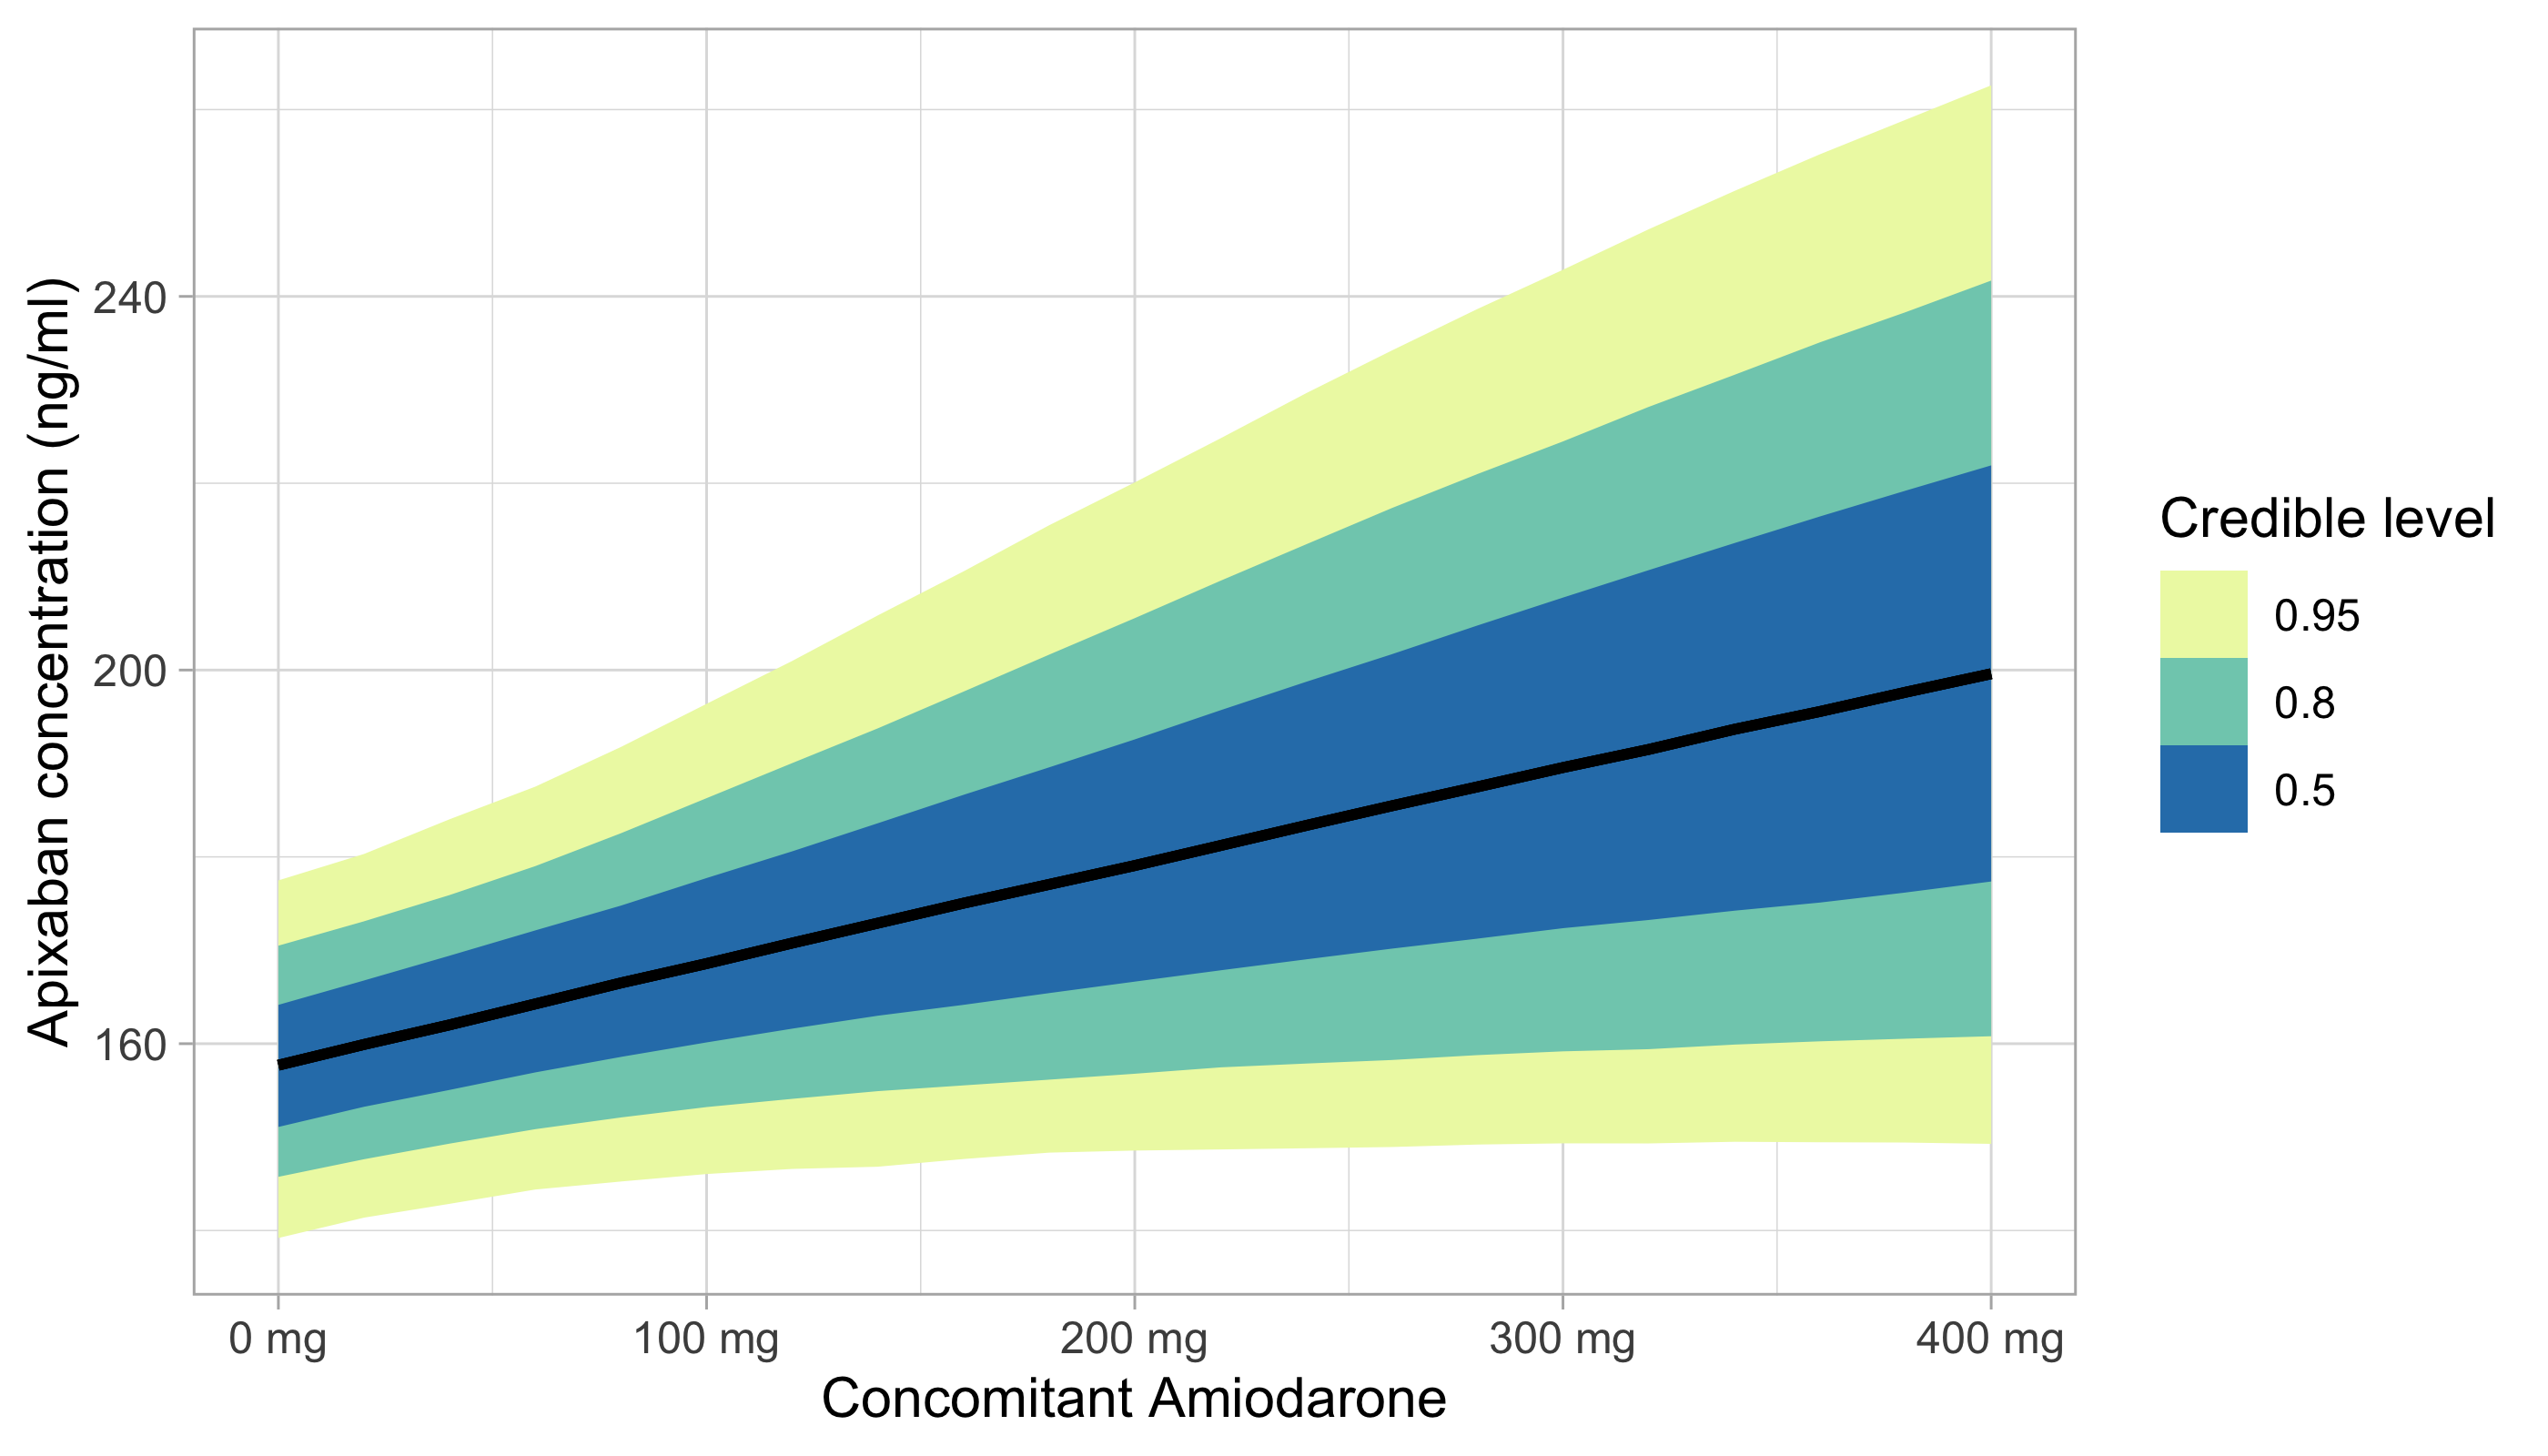
\includegraphics[width=\linewidth]{figures/max-concentration-1} 
		
	}
	
	\caption{Estimated max concentration as a function of concomitant amiodarone for a reference patient.  Concomitant amiodarone is estimated to increase apixaban bioavailability, thus leading to an increase in max concentration. The uncertainty in the effect of concomitant amiodarone is propagated through to the estimate of max concentration.  If max concentration is a key quantity in decision making, propagation of this uncertainty is crucial.}\label{fig:max-concentration}
\end{figure}

\begin{figure}
	
	{\centering 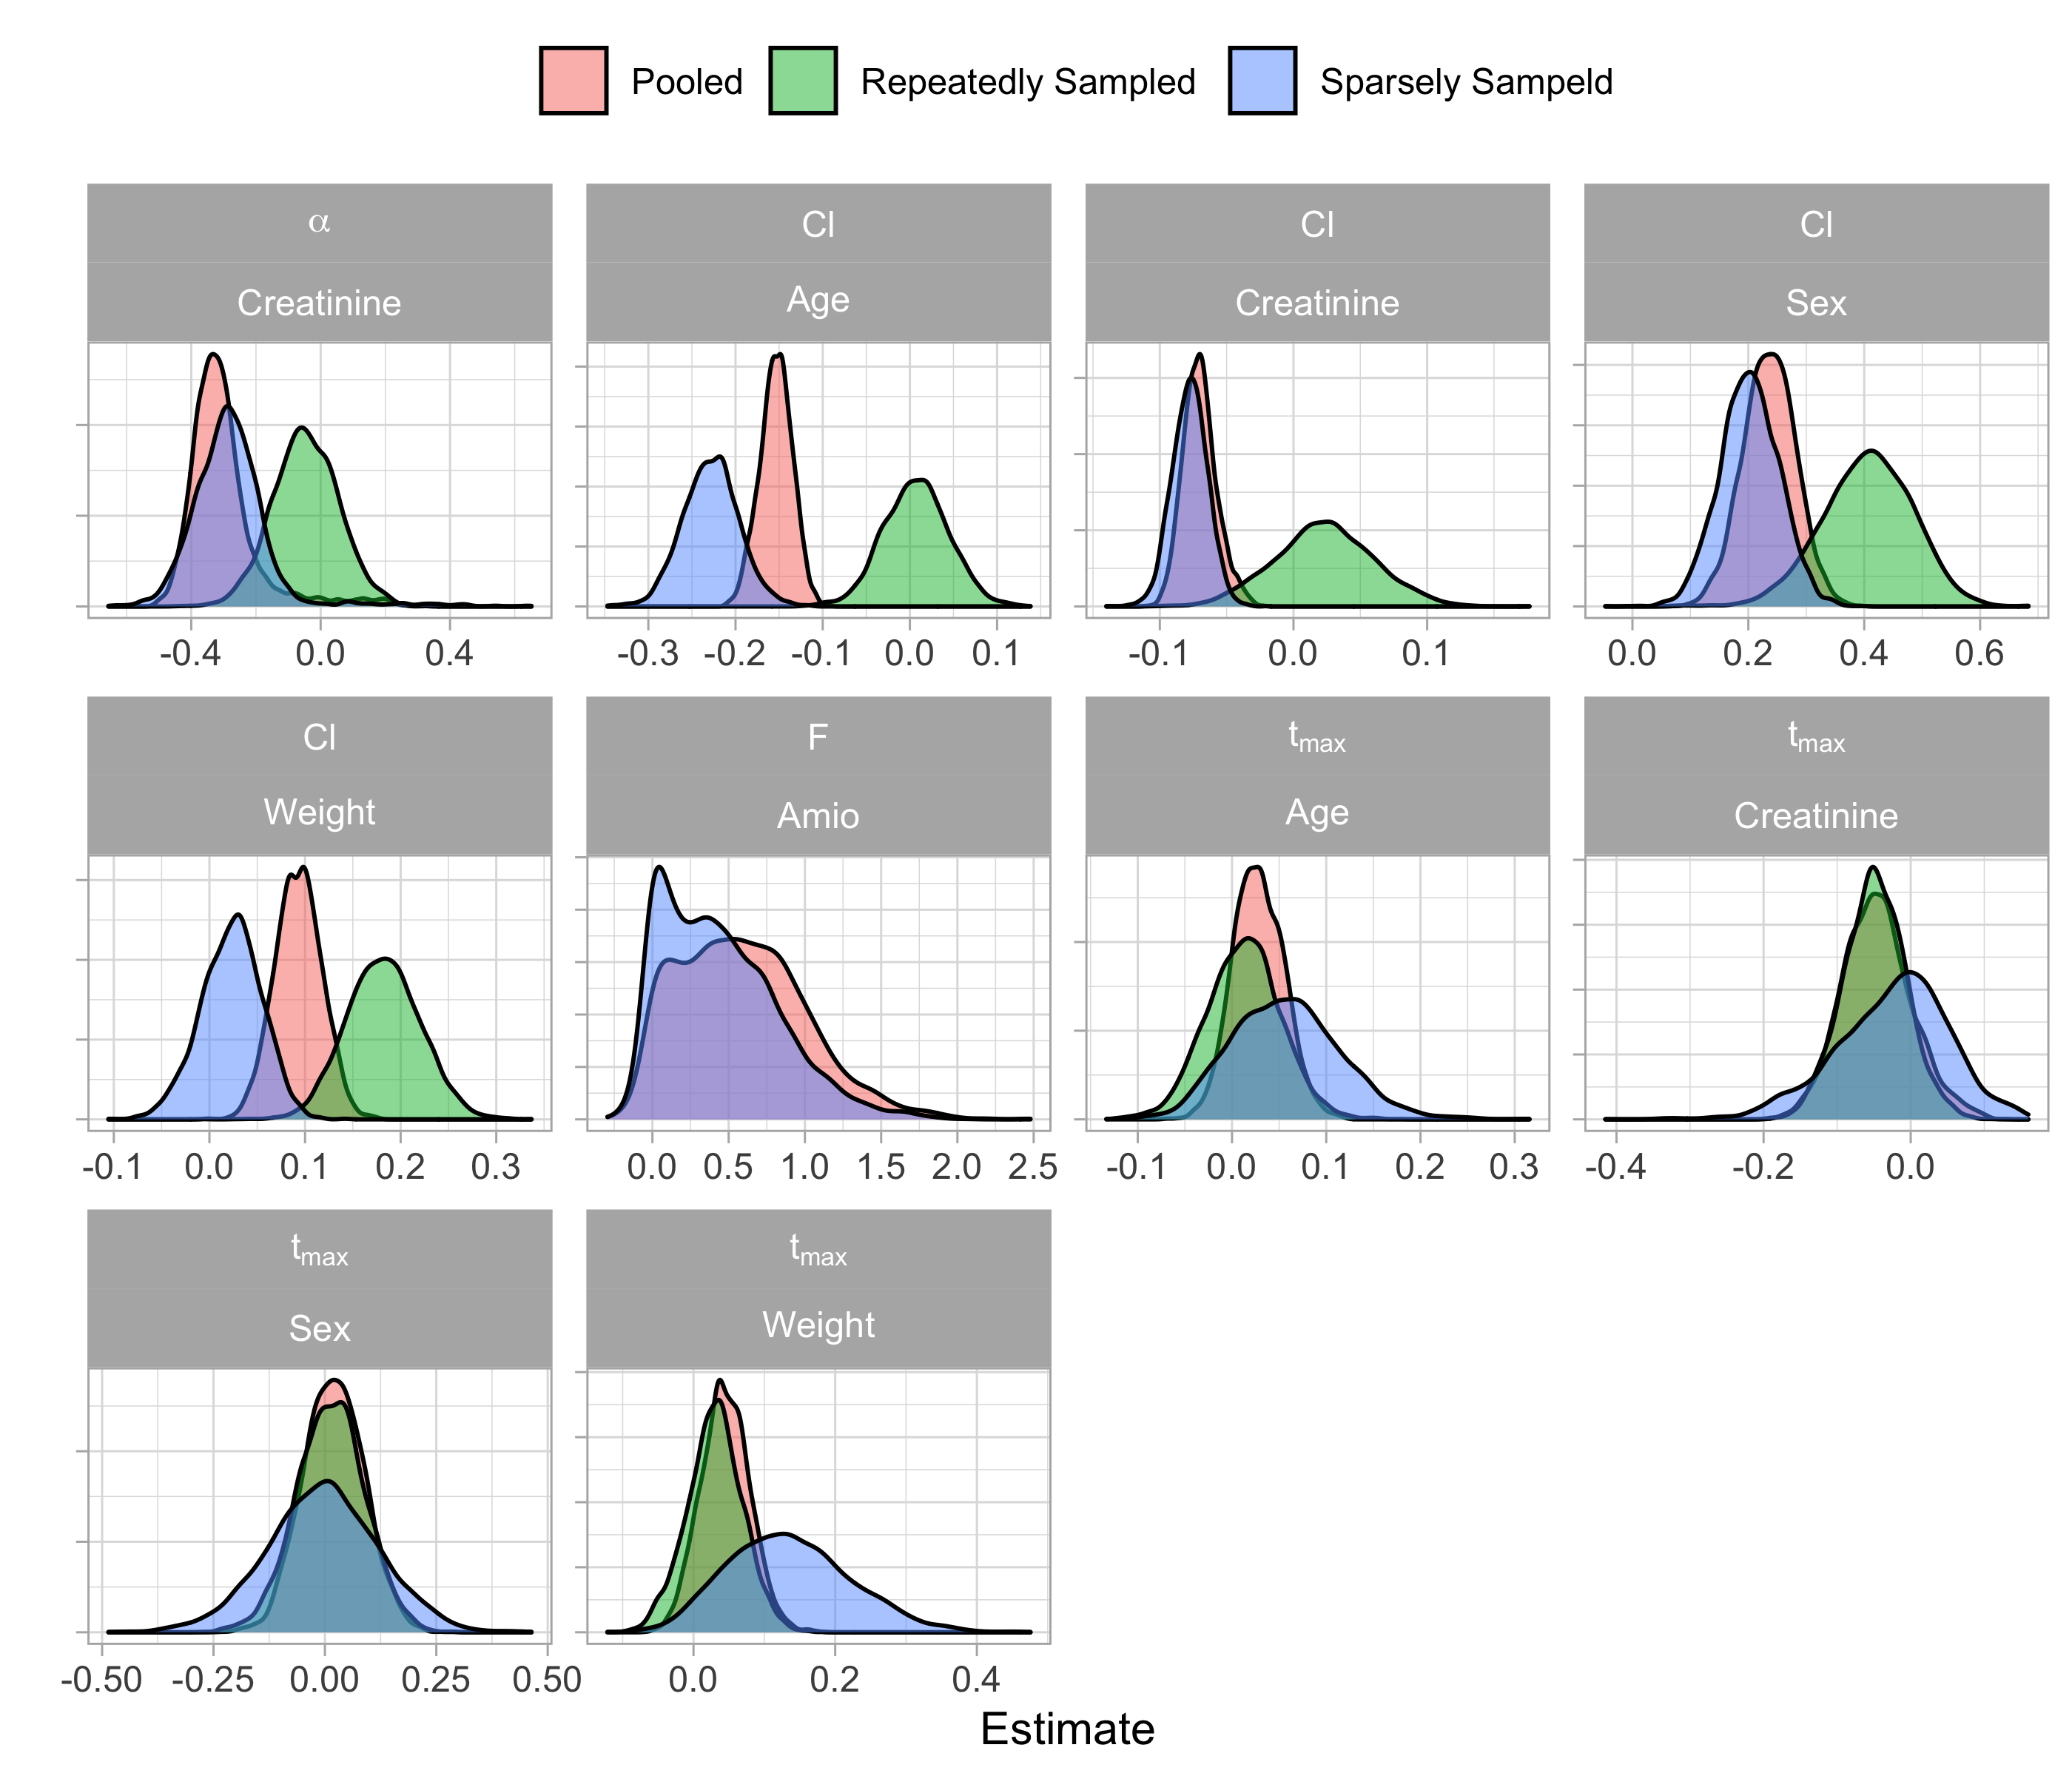
\includegraphics[width=\linewidth]{figures/effect-estimates-1} 
		
	}
	
	\caption{Estimated covariate effects from models fit to each dataset separately and the pooled model.}\label{fig:effect-estimates}
\end{figure}
